%
\documentclass[pdf,12pt]{article}

%\usepackage{times}
%\usepackage[FIGBOTCAP,normal,bf,tight]{subfigure}
\usepackage{amsmath}
\usepackage{amssymb}
%\usepackage{pifont}
\usepackage{enumerate}
\usepackage{listings}
\usepackage{fullpage}
\usepackage{xcolor}          % Using xcolor for more robust color specification
%\usepackage{ifthen}          % For simple checking in newcommand blocks
%\usepackage{textcomp}
%\usepackage{authblk}         % For making the author list look prettier
%\renewcommand\Authsep{,~\,}

% Custom colors
\definecolor{deepblue}{rgb}{0,0,0.5}
\definecolor{deepred}{rgb}{0.6,0,0}
\definecolor{deepgreen}{rgb}{0,0.5,0}
\definecolor{forestgreen}{RGB}{34,139,34}
\definecolor{orangered}{RGB}{239,134,64}
\definecolor{darkblue}{rgb}{0.0,0.0,0.6}
\definecolor{gray}{rgb}{0.4,0.4,0.4}

\lstset {
  basicstyle=\ttfamily,
  frame=single
}

\lstdefinestyle{XML} {
    language=XML,
    extendedchars=true,
    breaklines=true,
    breakatwhitespace=true,
%    emph={name,dim,interactive,overwrite},
    emphstyle=\color{red},
    basicstyle=\ttfamily,
%    columns=fullflexible,
    commentstyle=\color{gray}\upshape,
    morestring=[b]",
    morecomment=[s]{<?}{?>},
    morecomment=[s][\color{forestgreen}]{<!--}{-->},
    keywordstyle=\color{cyan},
    stringstyle=\ttfamily\color{black},
    tagstyle=\color{darkblue}\bf\ttfamily,
    morekeywords={name,type},
%    morekeywords={name,attribute,source,variables,version,type,release,x,z,y,xlabel,ylabel,how,text,param1,param2,color,label},
}
\lstset{language=xml}

\usepackage{titlesec}
\newcommand{\sectionbreak}{\clearpage}
\setcounter{secnumdepth}{4}


%%%%%%%% Begin comands definition to input python code into document
\usepackage[utf8]{inputenc}

% Default fixed font does not support bold face
\DeclareFixedFont{\ttb}{T1}{txtt}{bx}{n}{9} % for bold
\DeclareFixedFont{\ttm}{T1}{txtt}{m}{n}{9}  % for normal

\usepackage{listings}

% Python style for highlighting
%\newcommand\pythonstyle{\lstset{
%language=Python,
%basicstyle=\ttm,
%otherkeywords={self, none, return},             % Add keywords here
%keywordstyle=\ttb\color{deepblue},
%emph={MyClass,__init__},          % Custom highlighting
%emphstyle=\ttb\color{deepred},    % Custom highlighting style
%stringstyle=\color{deepgreen},
%frame=tb,                         % Any extra options here
%showstringspaces=false            %
%}}


% Python environment
%\lstnewenvironment{python}[1][]
%{
%$\pythonstyle
%\lstset{#1}
%}
%{}

% Python for external files
%\newcommand\pythonexternal[2][]{{
%\pythonstyle
%\lstinputlisting[#1]{#2}}}
%
%\lstnewenvironment{xml}
%{}
%{}

% Python for inline
%\newcommand\pythoninline[1]{{\pythonstyle\lstinline!#1!}}

%\def\DRAFT{} % Uncomment this if you want to see the notes people have been adding
% Comment command for developers (Should only be used under active development)
%\ifdefined\DRAFT
%  \newcommand{\nameLabeler}[3]{\textcolor{#2}{[[#1: #3]]}}
%\else
%  \newcommand{\nameLabeler}[3]{}
%\fi
% Commands for making the LaTeX a bit more uniform and cleaner
%\newcommand{\TODO}[1]    {\textcolor{red}{\textit{(#1)}}}
\newcommand{\xmlAttrRequired}[1] {\textcolor{red}{\textbf{\texttt{#1}}}}
\newcommand{\xmlAttr}[1] {\textcolor{cyan}{\textbf{\texttt{#1}}}}
\newcommand{\xmlNodeRequired}[1] {\textcolor{deepblue}{\textbf{\texttt{<#1>}}}}
\newcommand{\xmlNode}[1] {\textcolor{darkblue}{\textbf{\texttt{<#1>}}}}
\newcommand{\xmlString}[1] {\textcolor{black}{\textbf{\texttt{'#1'}}}}
\newcommand{\xmlDesc}[1] {\textbf{\textit{#1}}} % Maybe a misnomer, but I am
                                                % using this to detail the data
                                                % type and necessity of an XML
                                                % node or attribute,
                                                % xmlDesc = XML description
\newcommand{\default}[1]{~\\*\textit{Default: #1}}
\newcommand{\nb} {\textcolor{deepgreen}{\textbf{~Note:}}~}

% The bm package provides \bm for bold math fonts.  Apparently
% \boldsymbol, which I used to always use, is now considered
% obsolete.  Also, \boldsymbol doesn't even seem to work with
% the fonts used in this particular document...
\usepackage{bm}

% Define tensors to be in bold math font.
\newcommand{\tensor}[1]{{\bm{#1}}}

% Override the formatting used by \vec.  Instead of a little arrow
% over the letter, this creates a bold character.
\renewcommand{\vec}{\bm}

% Define unit vector notation.  If you don't override the
% behavior of \vec, you probably want to use the second one.
\newcommand{\unit}[1]{\hat{\bm{#1}}}

% Use this to refer to a single component of a unit vector.
\newcommand{\scalarunit}[1]{\hat{#1}}

% \toprule, \midrule, \bottomrule for tables
\usepackage{booktabs}

% \llbracket, \rrbracket
\usepackage{stmaryrd}

\usepackage{hyperref}

\usepackage{graphicx}
\graphicspath{{./figures/}}

% Compress lists of citations like [33,34,35,36,37] to [33-37]
\usepackage{cite}

% If you want to relax some of the SAND98-0730 requirements, use the "relax"
% option. It adds spaces and boldface in the table of contents, and does not
% force the page layout sizes.
% e.g. \documentclass[relax,12pt]{SANDreport}
%
% You can also use the "strict" option, which applies even more of the
% SAND98-0730 guidelines. It gets rid of section numbers which are often
% useful; e.g. \documentclass[strict]{SANDreport}

% The INLreport class uses \flushbottom formatting by default (since
% it's intended to be two-sided document).  \flushbottom causes
% additional space to be inserted both before and after paragraphs so
% that no matter how much text is actually available, it fills up the
% page from top to bottom.  My feeling is that \raggedbottom looks much
% better, primarily because most people will view the report
% electronically and not in a two-sided printed format where some argue
% \raggedbottom looks worse.  If we really want to have the original
% behavior, we can comment out this line...
\raggedbottom
\setcounter{secnumdepth}{5} % show 5 levels of subsection
\setcounter{tocdepth}{5} % include 5 levels of subsection in table of contents

% ---------------------------------------------------------------------------- %
%
% Set the title, author, and date
%
\title{The RAVEN PRA Plugin \\ - User Manual -}
%\author{%
%\begin{tabular}{c} Author 1 \\ University1 \\ Mail1 \\ \\
%Author 3 \\ University3 \\ Mail3 \end{tabular} \and
%\begin{tabular}{c} Author 2 \\ University2 \\ Mail2 \\ \\
%Author 4 \\ University4 \\ Mail4\\
%\end{tabular} }


\author{D. Mandelli, C. Wang, A. Alfonsi}

% There is a "Printed" date on the title page of a SAND report, so
% the generic \date should [WorkingDir:]generally be empty.
\date{\today}

%\def\component#1{\texttt{#1}}

% ---------------------------------------------------------------------------- %
%\newcommand{\systemtau}{\tensor{\tau}_{\!\text{SUPG}}}

% Added by Sonat
%\usepackage{placeins}
%\usepackage{array}

%\newcolumntype{L}[1]{>{\raggedright\let\newline\\\arraybackslash\hspace{0pt}}m{#1}}
%\newcolumntype{C}[1]{>{\centering\let\newline\\\arraybackslash\hspace{0pt}}m{#1}}
%\newcolumntype{R}[1]{>{\raggedleft\let\newline\\\arraybackslash\hspace{0pt}}m{#1}}

% end added by Sonat
% ---------------------------------------------------------------------------- %
%
% Start the document
%

\begin{document}
    \maketitle

    % ------------------------------------------------------------------------ %
    % The table of contents and list of figures and tables
    % Comment out \listoffigures and \listoftables if there are no
    % figures or tables. Make sure this starts on an odd numbered page
    %
    \cleardoublepage		% TOC needs to start on an odd page
    \tableofcontents
    %\listoffigures
    %\listoftables
    % ---------------------------------------------------------------------- %

    % ---------------------------------------------------------------------- %
    % This is where the body of the report begins; usually with an Introduction
    %
    \section{Introduction}
\label{sec:Introduction}

This document provides a detailed description of the PRA plugin for the RAVEN~\cite{RAVEN,RAVENtheoryMan} code.
The features included in this plugin are:
\begin{itemize}
	\item Event Tree (ET) Model (see Section~\ref{sec:ETModel}) 
	\item Fault Tree (FT) Model (see Section~\ref{sec:FTModel})
	\item Markov Model (see Section~\ref{sec:MarkovModel})
	\item Reliability Block Diagram (RBD) Model (see Section~\ref{sec:RBDmodel})
	\item Data Classifier (see Section~\ref{sec:dataClassifier})
	\item ET Data Importer (see Section~\ref{sec:ETdataImporter}) 
	\item FT Data Importer (see Section~\ref{sec:FTdataImporter})
\end{itemize}

    \section{ET Model}
\label{sec:ETModel}

This model is designed to read from file the structure of the ET and to import such Boolean logic structure as a RAVEN model.
The ET must be specified in a specific format: the OpenPSA format (\href{<url>}{https://github.com/open-psa}). 
As an example, the ET of Fig.~\ref{fig:ET} is translated in the OpenPSA format as shown below:

\begin{lstlisting}[style=XML,morekeywords={anAttribute},caption=ET of Fig.~\ref{fig:ET} in OpenPSA format., label=lst:ETModel]
<define-event-tree name="eventTree">
    <define-functional-event name="ACC"/>
    <define-functional-event name="LPI"/>
    <define-functional-event name="LPR"/>
    <define-sequence name="1"/>
    <define-sequence name="2"/>
    <define-sequence name="3"/>
    <define-sequence name="4"/>
    <initial-state>
        <fork functional-event="ACC">
            <path state="0">
                <fork functional-event="LPI">
                    <path state="0">
                        <fork functional-event="LPR">
                            <path state="0">
                                <sequence name="1"/>
                            </path>
                            <path state="+1">
                                <sequence name="2"/>
                            </path>
                        </fork>
                    </path>
                    <path state="+1">
                        <sequence name="3"/>
                    </path>
                </fork>
            </path>
            <path state="+1">
                <sequence name="4"/>
            </path>
        </fork>
    </initial-state>
</define-event-tree>
\end{lstlisting} 

\begin{figure}
    \centering
    \centerline{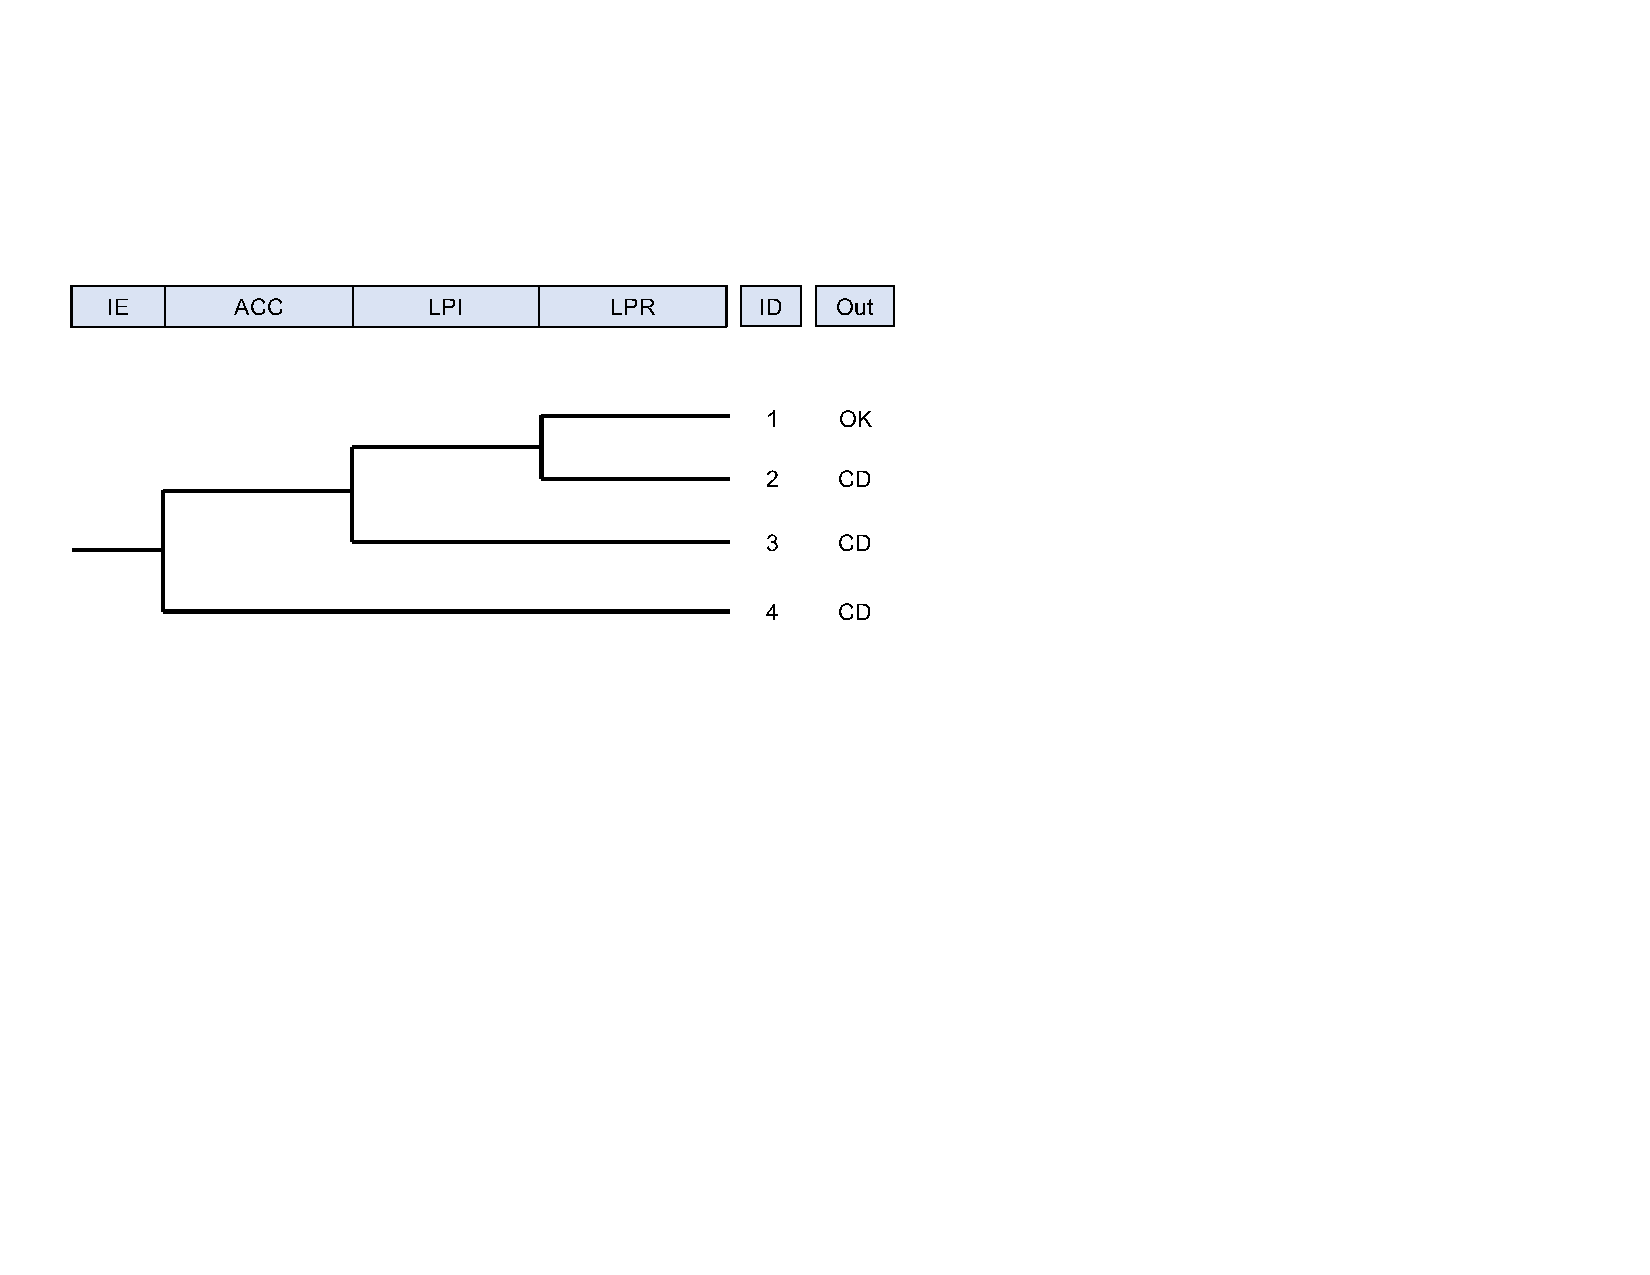
\includegraphics[scale=0.5]{ET.pdf}} 
    \caption{Example of ET.}
    \label{fig:ET}
\end{figure}

The ET of Fig.~\ref{fig:ET} and defined in Listing~\ref{lst:ETModel} can be defined in the RAVEN input file as follows:
\begin{lstlisting}[style=XML,morekeywords={anAttribute},caption=ET model input example., label=lst:ET_InputExample]
  <Models> 
    ...
    <ExternalModel name="ET" subType="ETModel">
      <variables>
        statusACC,statusLPI,statusLPR,sequence
      </variables>
      <map var="statusACC">ACC</map>
      <map var="statusLPI">LPI</map>
      <map var="statusLPR">LPR</map>
      <sequenceID>sequence</sequenceID>
    </ExternalModel>
    ...
  </Models>
\end{lstlisting}

All the specifications of the ET model are given in the 
\xmlNode{ExternalModel} block. 
Inside the \xmlNode{ExternalModel} block, the XML
nodes that belong to this models are:
\begin{itemize}
  \item  \xmlNode{variables}, \xmlDesc{string, required parameter}, a list containing the names of both the input and output variables of the model
  \item  \xmlNode{sequenceID},\xmlDesc{string, required parameter}, the name of the alias variable that indicate the branch ID
  \item  \xmlNode{map},\xmlDesc{string, required parameter}, the name ID of the ET branching variable
	  \begin{itemize}
	    \item \xmlAttr{var}, \xmlDesc{required string attribute}, the ALIAS name ID of the ET branching variable
	  \end{itemize}
\end{itemize}

Provided this definition and the ET model of Fig.~\ref{fig:ET} and described in Listing~\ref{lst:ETModel}, 
the resulting model in RAVEN is characterized by these variables:
\begin{itemize}
	\item Input variables: statusACC, statusLPI, statusLPR
	\item Output variable: sequence
\end{itemize}

\subsection{ET model reference tests}
\begin{itemize}
	\item test\_ETmodel.xml
	\item test\_ETmodel\_TD.xml
\end{itemize}




    \section{FT Model}
\label{sec:FTModel}

This model is designed to read from file the structure of the FT and to import such Boolean logic structure as a RAVEN model.
The FT must be specified in a specific format: the OpenPSA format (\href{<url>}{https://github.com/open-psa}). 
As an example, the FT of Fig.~\ref{fig:FT} is translated in the OpenPSA as shown below:

\begin{lstlisting}[style=XML,morekeywords={anAttribute},caption=FT in OpenPSA format., label=lst:FTModel]
<opsa-mef>
    <define-fault-tree name="FT">
        <define-gate name="TOP">
            <or>
                <gate name="G1"/>
                <gate name="G2"/>
                <gate name="G3"/>
            </or>
        </define-gate>
        <define-component name="A">
            <define-gate name="G1">
                <and>
                    <basic-event name="BE1"/>
                    <basic-event name="BE2"/>
                </and>
            </define-gate>
            <define-gate name="G2">
                <and>
                    <basic-event name="BE1"/>
                    <basic-event name="BE3"/>
                </and>
            </define-gate>
            <define-basic-event name="BE1">
                <float value="1.2e-3"/>
            </define-basic-event>
            <define-component name="B">
                <define-basic-event name="BE2">
                    <float value="2.4e-3"/>
                </define-basic-event>
                <define-basic-event name="BE3">
                    <float value="5.2e-3"/>
                </define-basic-event>
            </define-component>
        </define-component>
        <define-component name="C">
            <define-gate name="G3">
                <and>
                    <basic-event name="BE1"/>
                    <basic-event name="BE4"/>
                </and>
            </define-gate>
            <define-basic-event name="BE4">
                <float value="1.6e-3"/>
            </define-basic-event>
        </define-component>
    </define-fault-tree>
</opsa-mef>
\end{lstlisting} 

\begin{figure}
    \centering
    \centerline{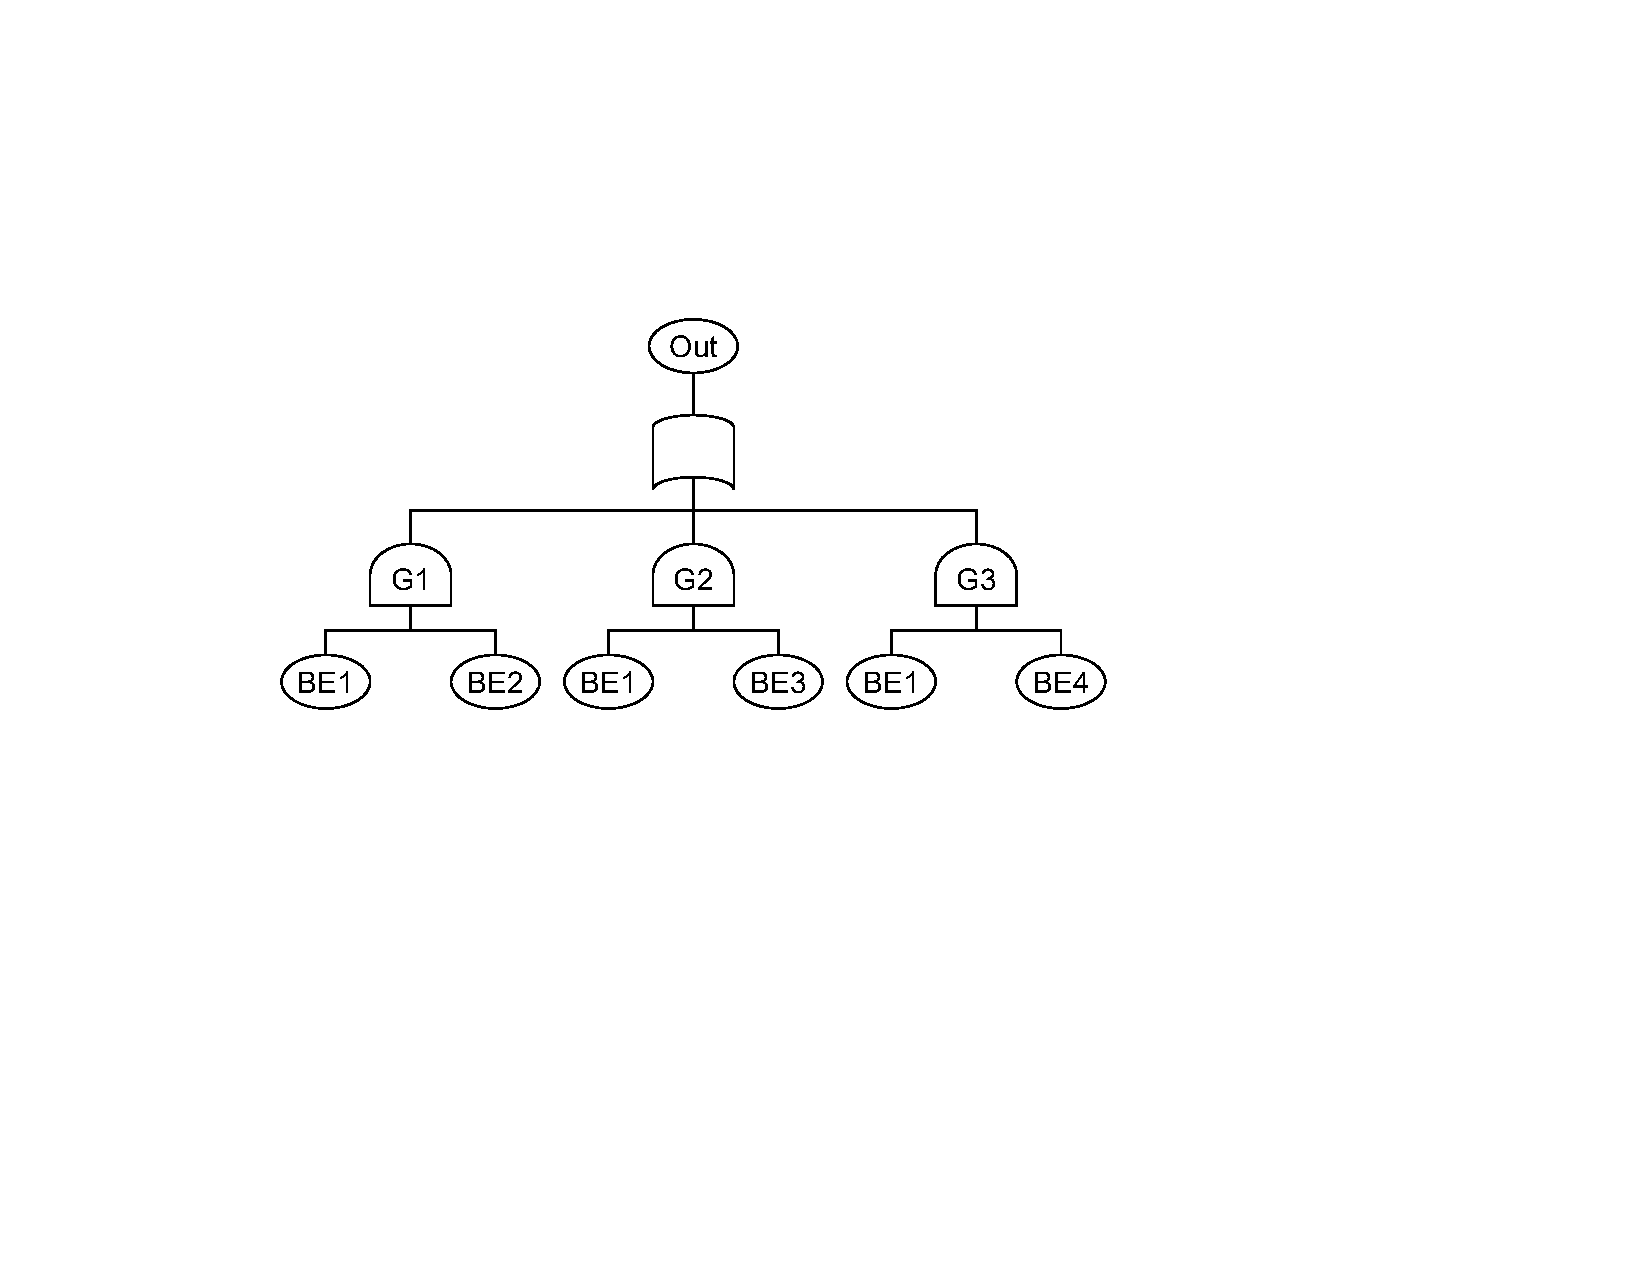
\includegraphics[scale=0.5]{FT.pdf}} 
    \caption{Example of FT.}
    \label{fig:FT}
\end{figure}

The FT of Fig.~\ref{fig:FT} and defined in Listing~\ref{lst:FTModel} can be defined in the RAVEN input file as follows:

\begin{lstlisting}[style=XML,morekeywords={anAttribute},caption=FT model input example., label=lst:FT_InputExample]
  <Models> 
    ...
    <ExternalModel name="FT" subType="FTModel">
      <variables>
        statusBE1,statusBE2,statusBE3,statusBE4,TOP
      </variables>
      <topEvents>TOP</topEvents>
      <map var="statusBE1">BE1</map>
      <map var="statusBE2">BE2</map>
      <map var="statusBE3">BE3</map>
      <map var="statusBE4">BE4</map>
    </ExternalModel>
    ...
  </Models>
\end{lstlisting}

All the specifications of the FT model are given in the 
\xmlNode{ExternalModel} block. 
Inside the \xmlNode{ExternalModel} block, the XML
nodes that belong to this models are:
\begin{itemize}
  \item  \xmlNode{variables}, \xmlDesc{string, required parameter}, a list containing the names of both the input and output variables of the model
  \item  \xmlNode{topEvents},\xmlDesc{string, required parameter}, the name of the alias Top Event
  \item  \xmlNode{map},\xmlDesc{string, required parameter}, the name ID of the FT basic events
	  \begin{itemize}
	    \item \xmlAttr{var}, \xmlDesc{required string attribute}, the ALIAS name ID of the FT basic events
	  \end{itemize}
\end{itemize}

Provided this definition, the FT model of Fig.~\ref{fig:ET} and described in Listing~\ref{lst:ETmodel}, 
the resulting model in RAVEN is characterized by these variables:
\begin{itemize}
	\item Input variables: statusBE1, statusBE2, statusBE3, statusBE4
	\item Output variable: TOP
\end{itemize}

\subsection{FT model reference tests}
\begin{itemize}
	\item test\_FTmodel.xml
	\item test\_FTmodel\_TD.xml
\end{itemize}

    \section{Markov Model}
\label{sec:MarkovModel}

This model is designed to import a generic Markov chain as a RAVEN model.
As an example, the Markov chain of Fig.~\ref{fig:markov} is translated in the OpenPSA as shown below:

\begin{figure}
    \centering
    \centerline{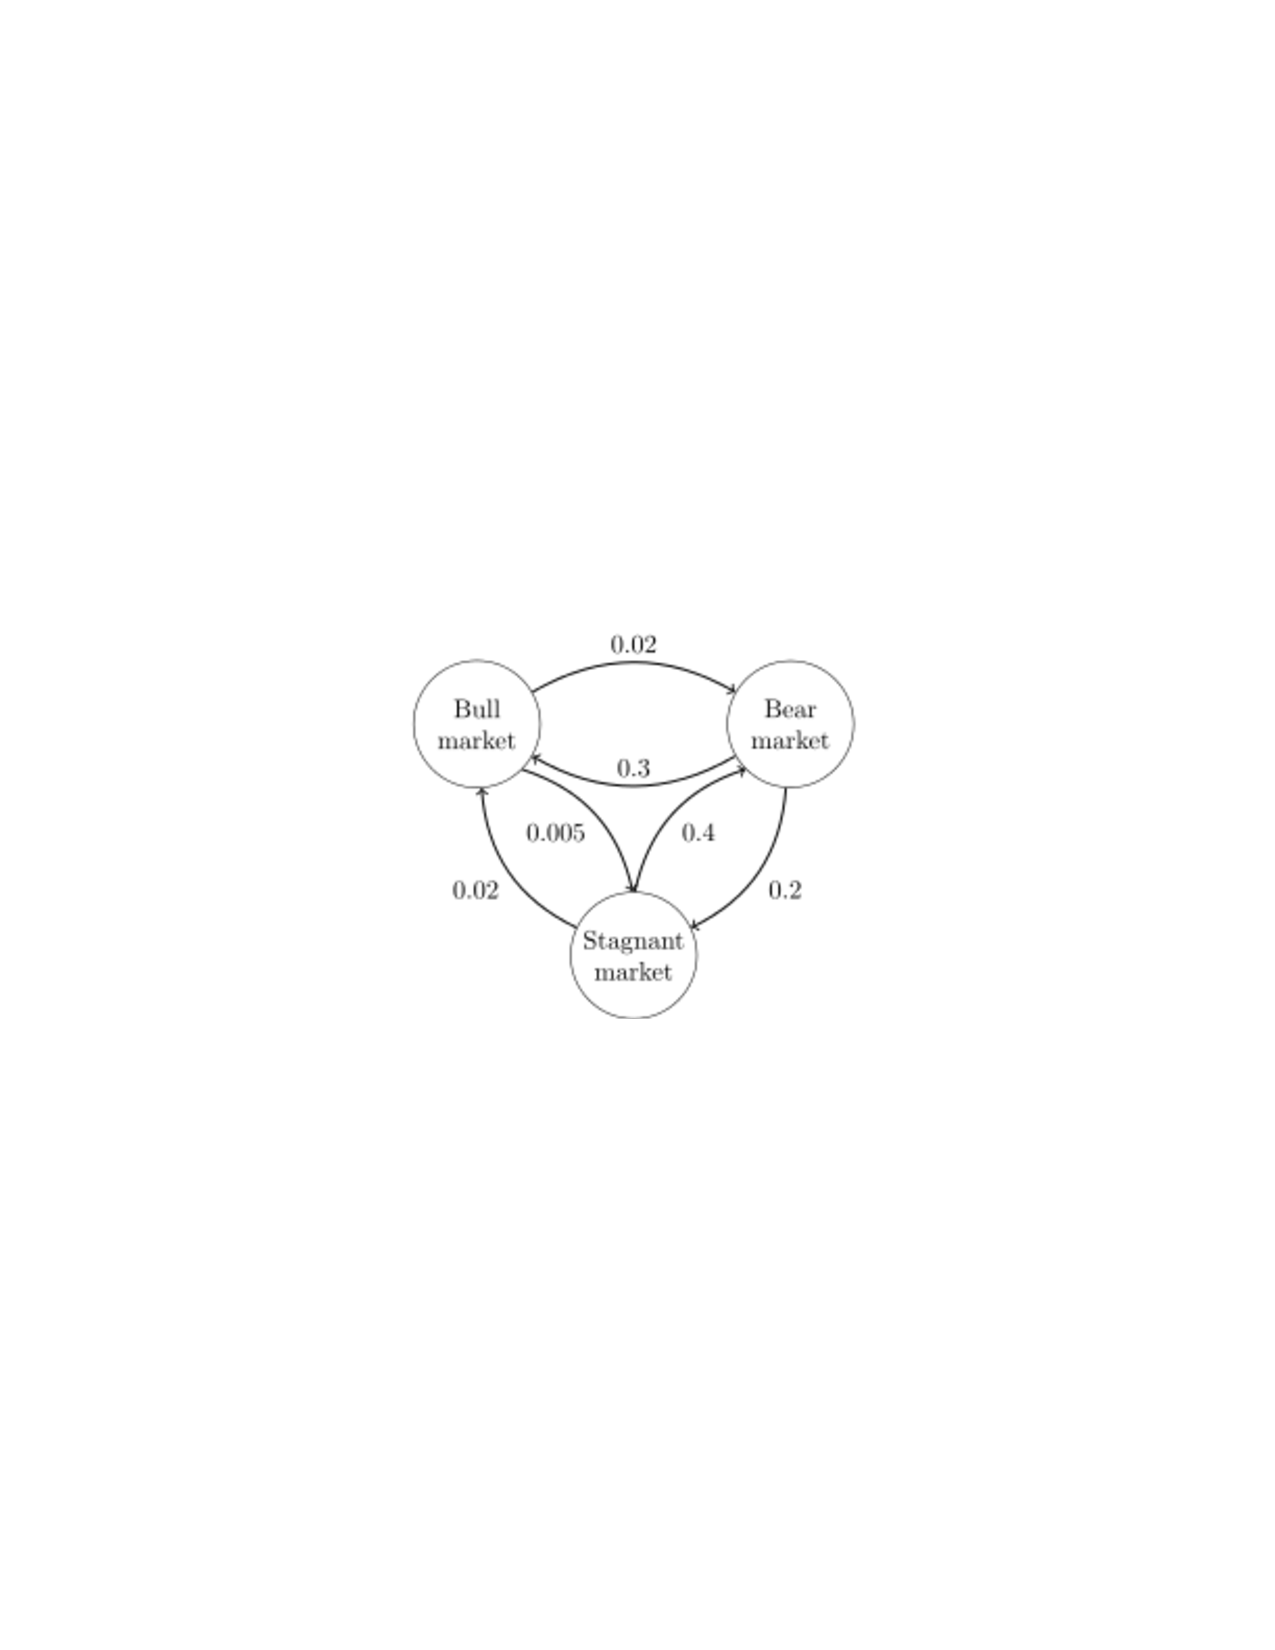
\includegraphics[scale=0.5]{markov.pdf}} 
    \caption{Example of continuous time Markov chain (source Wikipedia: https://en.wikipedia.org/wiki/Markov\_chain).}
    \label{fig:markov}
\end{figure}

\begin{lstlisting}[style=XML,morekeywords={anAttribute},caption=Markov model input example., label=lst:Markov_InputExample]
  <Models>
    <ExternalModel name="markov" subType="MarkovModel">
      <variables>initialState,finalState</variables>
      <initState>initialState</initState>
      <finState>finalState</finState>
      <endTime>1000</endTime>
      <state name="1"> <!-- Bull market -->
        <transition type="lambda" value="0.02" >2</transition>
        <transition type="lambda" value="0.005">3</transition>
      </state>
      <state name="2"> <!-- Bear market -->
        <transition type="lambda" value="0.3">1</transition>
        <transition type="lambda" value="0.2">3</transition>
      </state>
      <state name="3"> <!-- Stagnant market -->
        <transition type="lambda" value="0.02">1</transition>
        <transition type="lambda" value="0.4" >2</transition>
      </state>      
    </ExternalModel>
  </Models>
\end{lstlisting}

All the specifications of the Markov model are given in the \xmlNode{ExternalModel} block. 
Inside the \xmlNode{ExternalModel} block, the XML nodes that belong to this model are:
\begin{itemize}
  \item  \xmlNode{variables}, \xmlDesc{string, required parameter}, a list containing the names of both the input and output variables of the model
  \item  \xmlNode{initState}, \xmlDesc{string, required parameter}, variable ID corresponding to initial state
  \item  \xmlNode{finState}, \xmlDesc{string, required parameter}, variable ID corresponding to final state
  \item  \xmlNode{endTime}, \xmlDesc{float, required parameter}, time horizon to evaluate Markov chain transition history
  \item  \xmlNode{state}, specifies a single node; inside a \xmlNode{state} all possible transitions OUT of this state must be specified
                          in the \xmlNode{transition} xml sub-nodes:
	  \begin{itemize}
	  	\item \xmlAttr{transition}, \xmlDesc{required string attribute}, arrival state
	    \item \xmlAttr{type}, \xmlDesc{required string attribute}, type of transition. Allowed transition types are: The ET of Fig.~\ref{fig:ET} and defined in Listing~\ref{lst:ETmodel} can be defined in the RAVEN input file as follows: lambda, tau, instant and unif (see below)
	    \item \xmlAttr{value}, \xmlDesc{required string attribute}, value associated to the particular transition
	  \end{itemize}
\end{itemize}

The following transition types are available:
\begin{itemize}
  \item lambda: classical continuous time Markov chain transition rate in $\lambda$ form
  \item tau: classical continuous time Markov chain transition rate in the $\tau = \frac{1}{\lambda}$ form
  \item instant: deterministic transition out of particular state; the exact transition time is provided in input
  \item unif: transition time is uniformly sampled between the two provided values in the \xmlAttr{value} node
\end{itemize}

\subsection{Markov model reference tests}
\begin{itemize}
	\item test\_markovModel\_2states\_tau.xml
	\item test\_markovModel\_2states.xml
	\item test\_markovModel\_3states\_complexTrans.xml
	\item test\_markovModel\_3states\_instantTrans.xml
	\item test\_markovModel\_3states.xml
\end{itemize}

    \section{RBD Model}
\label{sec:RBDmodel}

This model is designed to read from file the structure of the RBD and import such Boolean logic structure as a RAVEN model.
The RBD must be specified in a specific format; as an example, the RBD of Fig.~\ref{fig:RBD} is translated in the RAVEN format as shown below:

\begin{lstlisting}[style=XML,morekeywords={anAttribute},caption=RBD input file., label=lst:RBDmodel]
<Graph name="testGraph">
  <node name="CST">
    <childs>1</childs>
  </node>
  <node name="1">
    <childs>2,3,4</childs>
  </node>
  <node name="2">
    <childs>5</childs>
  </node>
  <node name="3">
    <childs>5</childs>
  </node>
  <node name="4">
    <childs>5</childs>
  </node>
  <node name="5">
    <childs>6,7,8</childs>
  </node>
  <node name="6">
    <childs>SG1</childs>
  </node>
  <node name="7">
    <childs>SG2</childs>
  </node>
  <node name="8">
    <childs>SG3</childs>
  </node>
  <node name="SG1">
  </node>
  <node name="SG2">
  </node>
  <node name="SG3">
  </node>
</Graph>
\end{lstlisting} 

\begin{figure}
    \centering
    \centerline{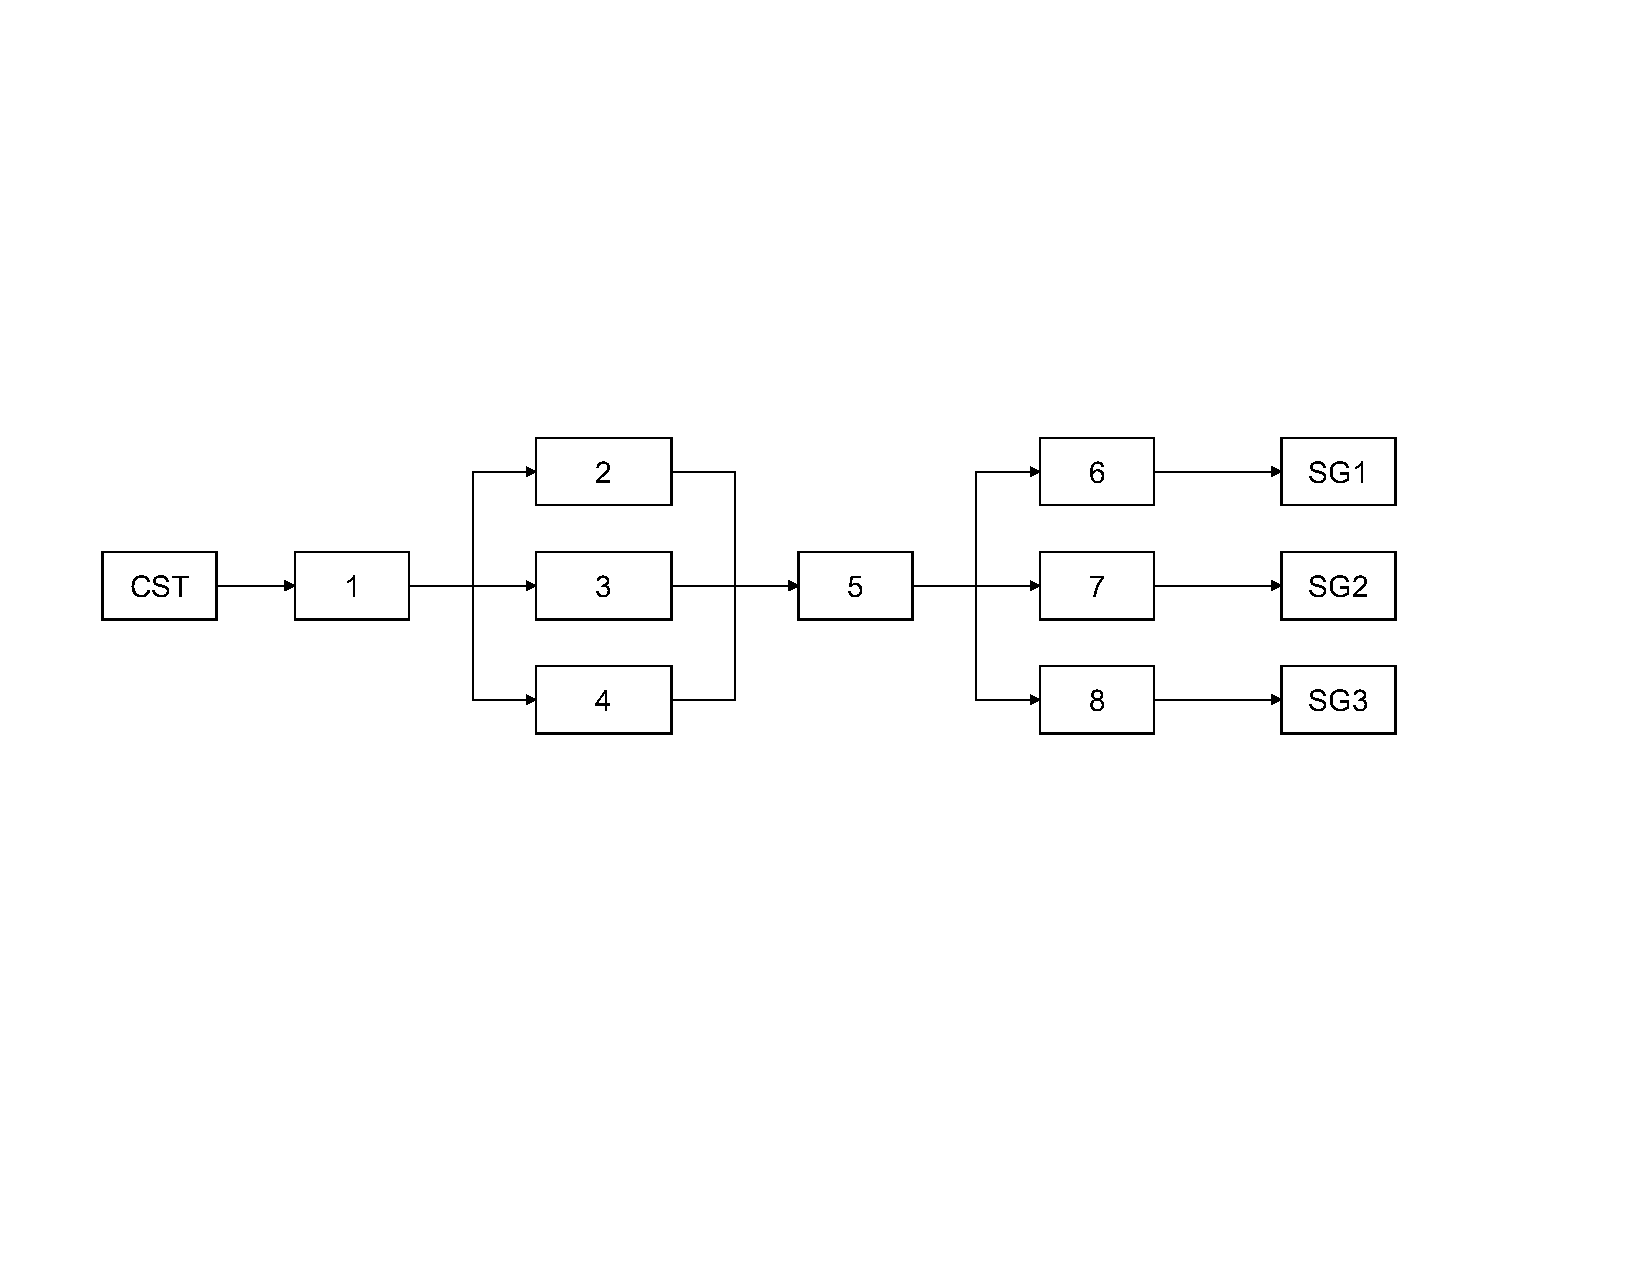
\includegraphics[scale=0.5]{RBD.pdf}} 
    \caption{Example of RBD.}
    \label{fig:RBD}
\end{figure}

The FT of Fig.~\ref{fig:RBD} and defined in Listing~\ref{lst:RBDmodel} can be defined in the RAVEN input file as follows:

\begin{lstlisting}[style=XML,morekeywords={anAttribute},caption=RBD model input example., label=lst:RBD_InputExample]
  <Models> 
    ...
    <ExternalModel name="graph" subType="GraphModel">
      <variables>
        status2,status3,status4,status5,
        statusSG1,statusSG2,statusSG3
      </variables>
      <modelFile>graphTest</modelFile>
      <nodesIN>CST</nodesIN>
      <nodesOUT>SG1,SG2,SG3</nodesOUT>
      <map var="status2">2</map>
      <map var="status3">3</map>
      <map var="status4">4</map>
      <map var="status5">5</map>
      <map var="statusSG1">SG1</map>
      <map var="statusSG2">SG2</map>
      <map var="statusSG3">SG3</map>
    </ExternalModel>
    ...
  </Models>
\end{lstlisting}

All the specifications of the RBD model are given in the 
\xmlNode{ExternalModel} block. 
Inside the \xmlNode{ExternalModel} block, the XML
nodes that belong to this models are:
\begin{itemize}
  \item  \xmlNode{variables}, \xmlDesc{string, required parameter}, a list containing the names of both the input and output variables of the model
  \item  \xmlNode{modelFile},\xmlDesc{string, required parameter}, the name of the file that provide the RBD structure
  \item  \xmlNode{nodesIN},\xmlDesc{string, required parameter}, the name of the input nodes
  \item  \xmlNode{nodesOUT},\xmlDesc{string, required parameter}, the name of the output nodes
  \item  \xmlNode{map},\xmlDesc{string, required parameter}, the name ID of the RBD node
	  \begin{itemize}
	    \item \xmlAttr{var}, \xmlDesc{required string attribute}, the ALIAS name ID of the RBD node
	  \end{itemize}
\end{itemize}

Provided this definition, the RBD model of Fig.~\ref{fig:RBD} and described in Listing~\ref{lst:RBDmodel}, 
the resulting model in RAVEN is characterized by these variables:
\begin{itemize}
	\item Input variables: status2, status3, status4, status5
	\item Output variable: statusSG1, statusSG2, statusSG3
\end{itemize}

\subsection{RBD model reference tests}
\begin{itemize}
	\item test\_graphModel.xml
	\item test\_graphModel\_TD.xml
\end{itemize}

    \section{Data Classifier}
\label{sec:dataClassifier}

The \textbf{DataClassifier} post-processor is specifically used to classify the data stored in the DataObjects. 
The details about this post-processors can be found in raven user manual subsection \textbf{PostProcessor}
of section \textbf{Models}.

\subsection{Data Classifier reference tests}
\begin{itemize}
	\item test\_dataClassifier\_postprocessor.xml
  \item test\_dataClassifier\_postprocessor\_HS.xml
\end{itemize}

    \section{ET Data Importer}
\label{sec:ETdataImporter}

This Post-Processor is designed to import an ET as a PointSet in RAVEN.
The ET must be specified in a specific format: the OpenPSA format (\href{<url>}{https://github.com/open-psa}). 
The details about this post-processors can be found in raven user manual subsection \textbf{PostProcessor}
of section \textbf{Models}.

\subsection{ET Importer reference tests}
\begin{itemize}
	\item test\_ETimporter.xml
	\item test\_ETimporterMultipleET.xml
	\item test\_ETimporterSymbolic.xml
	\item test\_ETimporter\_expand.xml
	\item test\_ETimporter\_DefineBranch.xml
	\item test\_ETimporter\_3branches.xml
	\item test\_ETimporter\_3branches\_NewNumbering.xml
	\item test\_ETimporter\_3branches\_NewNumbering\_expanded.xml
\end{itemize}

    \section{FT Data Importer}
\label{sec:FTdataImporter}

This Post-Processor is designed to import a FT as a PointSet in RAVEN.
The FT must be specified in a specific format: the OpenPSA format (\href{<url>}{https://github.com/open-psa}). 
The details about this post-processors can be found in raven user manual subsection \textbf{PostProcessor}
of section \textbf{Models}.

\subsection{FT Importer reference tests}
\begin{itemize}
	\item test\_FTimporter\_and\_withNOT\_embedded.xml
	\item test\_FTimporter\_and\_withNOT\_withNOT\_embedded.xml
	\item test\_FTimporter\_and\_withNOT.xml
	\item test\_FTimporter\_and.xml
	\item test\_FTimporter\_atleast.xml
	\item test\_FTimporter\_cardinality.xml
	\item test\_FTimporter\_component.xml
	\item test\_FTimporter\_doubleNot.xml
	\item test\_FTimporter\_iff.xml
	\item test\_FTimporter\_imply.xml
	\item test\_FTimporter\_multipleFTs.xml
	\item test\_FTimporter\_nand.xml
	\item test\_FTimporter\_nor.xml
	\item test\_FTimporter\_not.xml
	\item test\_FTimporter\_or\_houseEvent.xml
	\item test\_FTimporter\_or.xml
	\item test\_FTimporter\_xor.xml
\end{itemize}

    \section{MCSSolver}
\label{sec:MCSSolver}

This model is designed to read from file a list of Minimal Cut Sets (MCSs) and to import such Boolean logic structure as a RAVEN model.
Provided the sampled values of Basic Events (BEs) probabilities, the MCSSolver determines the probability of Top Event (TE), i.e., the union of the MCSs.
The list of MCS must be provided through a CSV file with the following format:

\begin{table}
  \begin{center}
    \caption{MCS file format.}
    \label{tab:table1}
    \begin{tabular}{c|c|c} 
      \textbf{ID} & \textbf{Prob} & \textbf{MCS}\\
      \hline
      1, & 0.01, & BE1\\
      2, & 0.02, & BE3\\
      3, & 0.03, & BE2,BE4\\
    \end{tabular}
  \end{center}
\end{table}

In this example:
\begin{itemize}
  \item three MCSs are defined: MCS1 = BE1, MCS2 = BE3 and MCS3 = BE2 and BE4 
  \item four BEs are defined: BE1, BE2, BE3 and BE4
  \item probability of TE, i.e. P(TE), is equal to: $P(TE) = P(MCS1 \cup MCS2 \cup MCS3)$
\end{itemize}

Note that the MCSSolver considers only the list of MCSs and it discards the rest of data contained in the csv file.

All the specifications of the MCSSolver model are given in the \xmlNode{ExternalModel} block. 
Inside the \xmlNode{ExternalModel} block, the XML nodes that belong to this models are:
\begin{itemize}
  \item  \xmlNode{variables}, \xmlDesc{string, required parameter}, a list containing the names of both the input and output variables of the model
  \item  \xmlNode{solverOrder},\xmlDesc{integer, required parameter}, solver order for $P(TE)$: it specifies the maximum calculation envelope 
                                                                      for $P(TE)$, i.e., the maximum number of MCSs to be considered when evaluating the 
                                                                      probability of their union
  \item  \xmlNode{topEventID},\xmlDesc{string, required parameter}, the name of the alias variable for the Top Event
  \item  \xmlNode{map},\xmlDesc{string, required parameter}, the name ID of the ET branching variable
	  \begin{itemize}
	    \item \xmlAttr{var}, \xmlDesc{required string attribute}, the ALIAS name ID of the basic event
	  \end{itemize}
\end{itemize}

An example of RAVEN input file is the following:

\begin{lstlisting}[style=XML,morekeywords={anAttribute},caption=MCSSolver model input example., label=lst:MCSSolver_InputExample]
  <Models> 
    ...
    <Models>
      <ExternalModel name="MCSmodel" subType="PRAplugin.MCSSolver">
        <variables>statusBE1,statusBE2,statusBE3,statusBE4,TOP</variables>
        <solverOrder>3</solverOrder>
        <topEventID>TOP</topEventID>>
        <map var='statusBE1'>BE1</map>
        <map var='statusBE2'>BE2</map>
        <map var='statusBE3'>BE3</map>
        <map var='statusBE4'>BE4</map>
      </ExternalModel>
    </Models>
    ...
  </Models>
\end{lstlisting}

If $solverOrder=1$ then: $P(TE) = P(MCS1)+P(MCS2)+P(MCS3)$.  
If $solverOrder=2$ then: $P(TE) = P(MCS1)+P(MCS2)+P(MCS3) - P(MCS1 MCS2) - P(MCS1 MCS3) - P(MCS2 MCS3)$.  
If $solverOrder=3$ then: $P(TE) = P(MCS1)+P(MCS2)+P(MCS3) - P(MCS1 MCS2) - P(MCS1 MCS3) - P(MCS2 MCS3) + P(MCS1 MCS2 MCS3)$

\subsection{MCSSolver model reference tests}
The following is the provided analytic test:
\begin{itemize}
	\item test\_MCSSolver.xml
\end{itemize}





    \section*{Document Version Information}
    This document has been compiled using the following version of the plug-in git repository:
    \newline
    d317572ffb80f564d27ec54e5db24d763705a8a5 Aaron Epiney - INL Tue, 17 Oct 2017 XX:XX:XX -0600


    % ---------------------------------------------------------------------- %
    % References
    %
    \clearpage
    % If hyperref is included, then \phantomsection is already defined.
    % If not, we need to define it.
    \providecommand*{\phantomsection}{}
    \phantomsection
    \addcontentsline{toc}{section}{References}
    \bibliographystyle{ieeetr}
    \bibliography{user_manual}


    % ---------------------------------------------------------------------- %

\end{document}
